\chapter{シミュレータの実装}
\label{implementation}
本提案手法の妥当性を検討する評価実験を行うために,シミュレータを実装した.
本章では本シミュレータの構成と,モデルケースとする慶應義塾大学湘南藤沢キャンパスの駐車場環境について概説にする.
\section{設計}
本シミュレータは,事前に作成した仮想地図上を仮想車両群が走行し,各車両の位置情報の履歴のみを用いてネットワークモデルの推定を行うものである.

\subsection{地図について}
\label{map-implementation}
本シミュレータでは仮想地図を$Map$クラスとして実装する.表\ref{map-class}に主要なプロパティとメソッドを列挙する.


\begin{table}[htbp]
	\centering
	\resizebox{\textwidth}{!}{%
		\begin{tabular}{ll}
			\hline
			\multicolumn{2}{c}{class Map} \\ \hline
			\multicolumn{1}{c|}{プロパティ名} & \multicolumn{1}{c}{概要}                                                                                                         \\ \hline
			\multicolumn{1}{l|}{places}             & 保有するPlaceインスタンスの配列                                                                                       \\
			\multicolumn{1}{l|}{parkings}           & 保有するPlacesインスタンスの中で,駐車区画であるものの配列                                               \\
			\multicolumn{1}{l|}{graph}              & networkxのGraphインスタンス                                                                                                 \\
			\multicolumn{1}{l|}{paths}              & すべてのノードからノードへの最短経路を収納した二次元配列                                               \\ \hline
			\multicolumn{1}{c|}{メソッド名}    & \multicolumn{1}{c}{概要}                                                                                                         \\ \hline
			\multicolumn{1}{l|}{genJson}            & 事前に作成した地図の構成を記したJSON形式のテキストファイルからMapインスタンスを初期化する \\
			\multicolumn{1}{l|}{choiceDest}         & placesに記録された人気度からCarインスタンスの目的地となるPlaceインスタンスを返す                  \\ \hline
		\end{tabular}%
	}
	\caption{地図を表す$Map$クラス}
	\label{map-class}
\end{table}


\subsection{ノードとエッジ}
$Map$インスタンスは,駐車区画や交差点を示す``ノード'',それらを結ぶ道路を示す``エッジ''によって構成された重み付きグラフとして表現される.これは本研究の提案手法で推定するネットワークモデルと同一のものを示す.各要素の位置関係や接続関係はNetworkX\footnote{ネットワークグラフを扱うライブラリ.\url{https://networkx.github.io/}}によって実装する.

\subsubsection{ノード}
ネットワークモデルにおいて駐車区画及び交差点を表す``ノード''は$Place$クラスとして実装される.表\ref{place-class}に$Place$クラスの主要なプロパティとメソッドを列挙する.


$Place$クラスは緯度$\cdot$経度によって表現される位置情報($XY$プロパティ)を有する.本シミュレータではその情報に伴って仮想車両の位置情報が決定される.このフローに関しては第\ref{car-implementation}項にて詳細に記述する.

また,各$Place$インスタンスには保有する駐車枠数の情報が付与される.これは仮想車両が駐車$\cdot$移動を行う度に増減する.

加えて,各インスタンスには人気度($popularity$プロパティ)を付与する.この人気度に則って車両の目的地が決定される.


\begin{table}[htbp]
	\centering
	\resizebox{\textwidth}{!}{%
		\begin{tabular}{ll}
			\hline
			\multicolumn{2}{c}{class Place} \\ \hline
			\multicolumn{1}{c|}{プロパティ名} & \multicolumn{1}{c}{概要}                                                                                       \\ \hline
			\multicolumn{1}{l|}{id\_}               & Mapインスタンスが持つPlaceインスタンスを一意に決定する                                    \\
			\multicolumn{1}{l|}{capacity}           & Placeインスタンス上に駐車可能な車両の数 交差点のインスタンスには0が挿入される \\
			\multicolumn{1}{l|}{availability}       & 現在の空き駐車枠の数 交差点のインスタンスには0が挿入される                           \\
			\multicolumn{1}{l|}{isfull}             & 満車かどうかを表す 交差点のインスタンスではFalseが常に入る                             \\
			\multicolumn{1}{l|}{XY}                 & Placeインスタンスの位置情報を(経度,緯度)の配列で示す                                     \\
			\multicolumn{1}{l|}{popularity}         & 駐車区画の人気度を示す値 0〜100の整数が入る                                                   \\
			\multicolumn{1}{l|}{passage\_cars}      & 通過しているCarインスタンスが挿入される配列                                                  \\
			\multicolumn{1}{l|}{parking\_cars}      & 駐車しているCarインスタンスが挿入される配列                                                  \\ \hline
			\multicolumn{1}{c|}{メソッド名}    & \multicolumn{1}{c}{概要}                                                                                       \\ \hline
			\multicolumn{1}{l|}{add\_passage}       & 車両が通過している際に実行される                                                                 \\
			\multicolumn{1}{l|}{add\_park}          & 車両が駐車しようとしている際に実行される 駐車の可否をbool型で返す                  \\
			\multicolumn{1}{l|}{remove\_car}        & 車両がこのインスタンス上から立ち去る際に実行される                                      \\ \hline
		\end{tabular}%
	}
	\caption{駐車区画$\cdot$交差点を表す$Place$クラス}
	\label{place-class}
\end{table}

\subsubsection{エッジ}
道路を表すエッジは$Place$インスタンス間を1:1の関係で結ぶ.エッジには距離を表す指数``weight''が付与されている.本シミュレータでは,先に述べたNetworkXのEdgeインスタンスとして表現する.


\subsection{車両について}
\label{car-implementation}
本実装では仮想車両を$Car$クラスとして表現する.本シミュレータでは複数の$Car$インスタンスを作成し,移動ログデータを記録$\cdot$解析する.
図\ref{car-class}に$Car$クラスの主要なプロパティとメソッドを記述する.


\begin{table}[htbp]
	\centering
	\resizebox{\textwidth}{!}{%
		\begin{tabular}{ll}
			\hline
			\multicolumn{2}{c}{class Car} \\ \hline
			\multicolumn{1}{c|}{プロパティ名} & \multicolumn{1}{c}{概要}                                                                                               \\ \hline
			\multicolumn{1}{l|}{id\_}               & Simulatorインスタンスが持つCarインスタンスを一意に決定する                                        \\
			\multicolumn{1}{l|}{firstplace}         & Carインスタンスが生成された時に現在地とするPlaceインスタンス                                   \\
			\multicolumn{1}{l|}{destination}        & 目的地となるPlaceインスタンスのid\_                                                                         \\
			\multicolumn{1}{l|}{confusion}          & destinationではない駐車区画を通過する際に駐車を強行する確率 0〜1のfloat型                     \\
			\multicolumn{1}{l|}{path}               & destinationまでの最短経路 Mapインスタンスが持つpathから取得する                                    \\
			\multicolumn{1}{l|}{isparked}           & 駐車しているかどうかを表す bool型                                                                          \\
			\multicolumn{1}{l|}{parking\_counter}   & 駐車するシーケンス数 Simulatorクラスで定められた範囲内で決定される int型                    \\
			\multicolumn{1}{l|}{position}           & 現在居るPlaceインスタンス                                                                                      \\
			\multicolumn{1}{l|}{XY}                 & 現在居る位置情報が(経度,緯度)の配列で挿入される                                                  \\
			\multicolumn{1}{l|}{isonedge}           & 現在道路上(エッジ)にいるかどうか bool型                                                                  \\
			\multicolumn{1}{l|}{error}              & 位置情報の誤差の大きさを決定する値 float型                                                             \\ \hline
			\multicolumn{1}{c|}{メソッド名}    & \multicolumn{1}{c}{概要}                                                                                               \\ \hline
			\multicolumn{1}{l|}{setPath}            & 目的地までの経路を生成しpathに代入する                                                                  \\
			\multicolumn{1}{l|}{nextseq}            & この車両のシーケンスを進める 下記の各メソッドを実行する                                       \\
			\multicolumn{1}{l|}{move\_to}           & 次に移動するPlaceインスタンスを引数に取り,Carインスタンスのプロパティの編集する     \\ \hline
			\multicolumn{1}{l|}{arrive\_at}         & 新しいPlaceインスタンスに到着した時に実行される                                                     \\
			\multicolumn{1}{l|}{try\_park\_at}      & 駐車区画のPlaceインスタンスに到着した際に駐車を試みる 成功の可否をbool型で返す         \\
			\multicolumn{1}{l|}{park\_at}           & try\_park\_atで駐車が成功した際に実行される                                                               \\
			\multicolumn{1}{l|}{calcPosition}       & \begin{tabular}[c]{@{}l@{}}毎シーケンスごとに位置情報をSimulatorインスタンスに渡すための関数 \\ errorの値に基づいて誤差を生成する\end{tabular} \\ \hline
		\end{tabular}%
	}
	\caption{仮想車両を表す$Car$クラス}
	\label{car-class}
\end{table}
\subsubsection{$Car$インスタンスの振る舞い}
本項ではシミュレータ上における$Car$インスタンスの振る舞いについて記述する.
$Car$インスタンスは1シーケンスが進むごとに仮想地図内を移動していく.その過程を図\ref{car-implementation-flow}に示す.

\begin{figure}
	\centering
	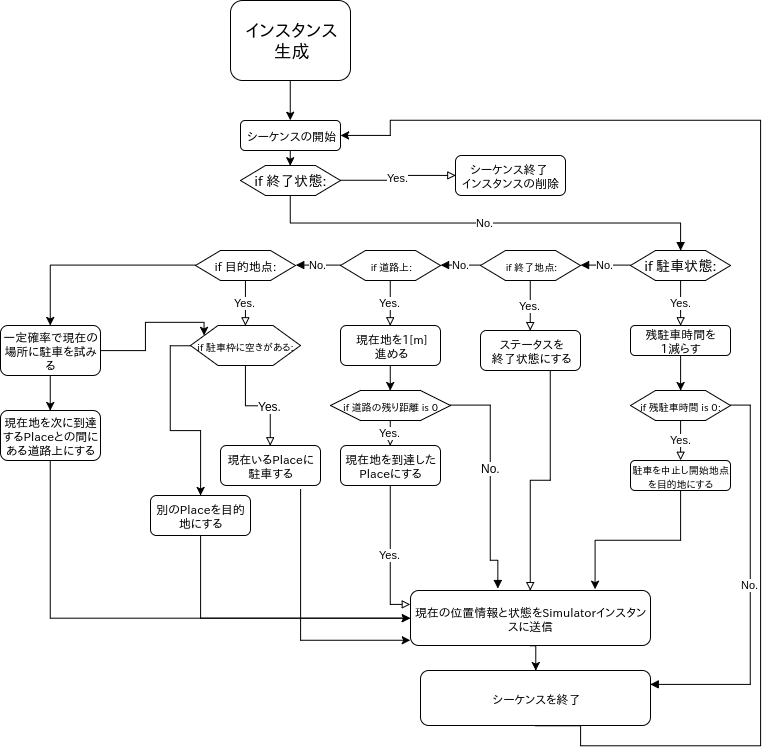
\includegraphics[width=14cm]{fig/car-implementation-flow.png}
	\caption{1シーケンス中の$Car$インスタンスの振る舞いを表す図}
	\label{car-implementation-flow}
\end{figure}

車両は1シーケンスごとに定められた台数が場内に進入する.
この時の開始地点は$Map$インスタンスが持つ$Place$の内$id\_=0$の地点とする.
各車両は識別コード($id\_$)の若い車両から順番に,1シーケンスごとに進入$\cdot$移動$\cdot$駐車$\cdot$退出を行う.

\begin{itemize}
	\item 移動 \\
	      場内に進入した車両は,それぞれに固有に与えられた目的地を目指して,定められた経路に則って移動する.なお,本シミュレータではダイクストラ法\cite{Dijkstra}を用いて最短経路を計算する.
	      エッジ上を移動している車両は1シーケンスごとに1[m]を移動する.車両の移動速度$v$は$v=1$[m/s]である.
	\item 駐車 \\
	      目的地となる駐車区画に到着した車両は必ず駐車を試みる.既に駐車している車両で駐車枠が占領されている場合,再度目的地の設定を行う.この時,同様に経路も再設定される.以後駐車が成功するまでこれを繰り返す.駐車に成功した場合,事前に定められたシーケンス数$parking_counter$だけ駐車する.この駐車時間$parking_counter$は1試行ごとに設定された範囲内(1時間〜3時間)の任意の時間である.駐車開始時に送信される位置情報には,駐車中を表すフラグが付与される.なお,駐車中にはエンジンが停止しており機器の電源が切られていると想定し,$Car$インスンタンスは位置情報の送信を行わない.駐車終了後.発進を表すフラグを付与した位置情報を送信した後に.次のシーケンスより開始地点を目的地にした移動を開始する.
	\item 退出 \\
	      駐車終了後に開始地点に帰還した$Car$インスタンスは$Simulator$クラスから削除される.
\end{itemize}
\subsubsection{位置情報の送信}
\label{implementation-send-position}
$Car$インスタンスは1シーケンスごとに位置情報を記録したメッセージを$Simulator$クラスに送信する.
以下が$Car$インスタンス$C$が送信するメッセージ$M$のフォーマットである.
\begin{align}
	M = \left(I_C,S_C,G_C\right) \\
	I_C = Cの識別id               \\
	S_C = Cの現在の状態        \\
	G_C = Cの位置情報
\end{align}


ノード上に車両が存在している場合はそのノードの位置情報を,エッジ上に存在している場合はノード間の位置情報をエッジの重みで分割した値が送信される.なお,ノード間の距離は計算量の削減のためにユークリッド距離\cite{cluster-analysis}で求める.
$Place$インスタンス$P_a$上の$Car$インスタンスの位置情報$G_C$は以下の式で表される.
\begin{align}
	G_C = g(x),x = G_a                    \\
	g(x) = 誤差関数                       \\
	G_a = P_aの位置情報(経度,緯度) \\
\end{align}

$Place$インスタンス$P_a \cdot P_a$間に位置するエッジ$E$に進入した$Car$インスタンスの位置情報$G_E$は以下の式で表される.
\begin{align}
	G_E = g(x),x = \frac{\sqrt{\sum{\left(G_a - G_b\right)^2}} \cdot t_n}{E_w} \\
	g(x) = 誤差関数                                                          \\
	G_a = P_1の位置情報(経度,緯度)                                    \\
	G_b = P_2の位置情報(経度,緯度)                                  \\
	t_n = CがEに進入してからの経過シーケンス                     \\
	E_w = Eの重さ(距離)                                                     
\end{align}

各$Car$インスタンスが送信する位置情報には,実際の衛星測位システムの誤差\cite{gps-gov}を模した最大+-10[m]程度の誤差付与処理を行う.
安田の調査\cite{Yasuda}によれば,位置情報測位システムによる誤差は正規分布のため,本実装の誤差付与処理では結果を正規分布させる.以下が本実装における誤差を付与する誤差関数$g(x)$を表す式である.

\begin{align}
	g(x) = x  + \frac{R}{10^{4.5}}                                        \\
	x = 位置情報の真値                                               \\
	R = 標準正規分布(平均0,標準偏差1)の乱数を返す関数 
\end{align}

予備実験として,誤差関数$g(x)$を1000回実行した.この時の位置情報の真値との距離の分布と密度を図\ref{error-kde}に示す.なお,$x$は第\ref{evaluation}章にて評価実験を行う慶應義塾大学湘南藤沢キャンパスの座標を選択した.2点間の距離の計算にはGeoPy\footnote{地球上の二組の座標から距離を割り出すことが出来るライブラリ.\url{https://github.com/geopy/geopy}}を利用した.

\begin{figure}
	\centering
	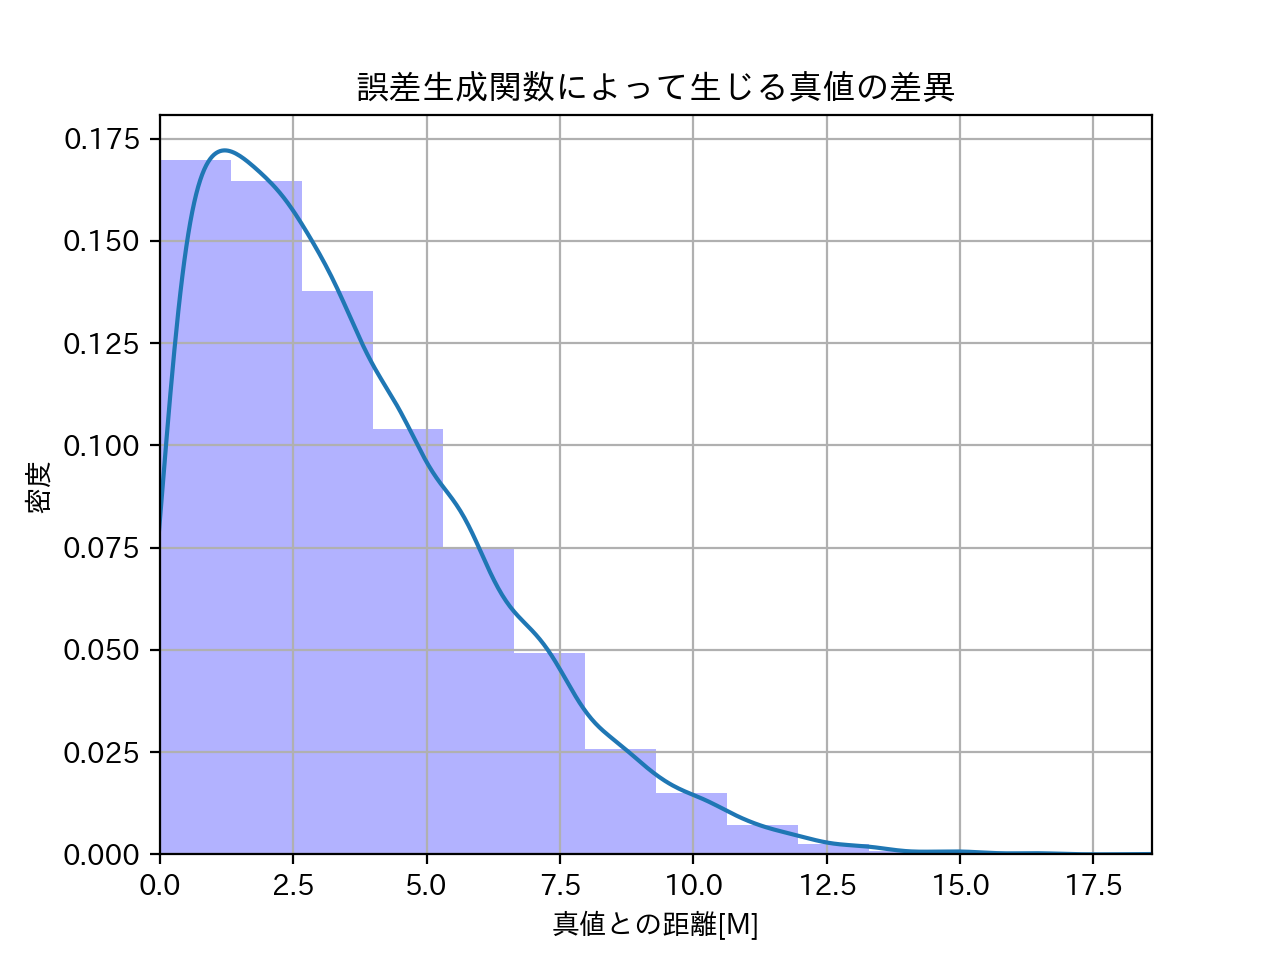
\includegraphics[width=13cm]{fig/error_kde.png}
	\caption{誤差関数$g(x)$が返す位置情報と真値との差分の分布を表すヒストグラム}
	\label{error-kde}
\end{figure}

\subsection{時間経過と評価実験プログラムについて}
本実装では,$Simulator$クラスが仮想地図と仮想車両を管理し,シミュレーションの進行を担う.
図\ref{simulator-class}に主要なプロパティとメソッドを記述する.

\begin{table}[htbp]
	\centering
	\resizebox{\textwidth}{!}{%
		\begin{tabular}{ll}
			\hline
			\multicolumn{2}{c}{class Simulator} \\ \hline
			\multicolumn{1}{c|}{プロパティ名}       & \multicolumn{1}{c}{概要}                                                                                                          \\ \hline
			\multicolumn{1}{l|}{sequence}                 & 現在のシーケンスが挿入される int型                                                                                   \\
			\multicolumn{1}{l|}{map}                      & Simulatorインスタンスが保有するMapインスタンス                                                                     \\
			\multicolumn{1}{l|}{cars}                     & Simulatorインスタンスが保有するCarインスタンスが挿入される配列                                             \\
			\multicolumn{1}{l|}{car\_pace}                & isgradulalyがTrueの場合にCarインスタンスを作成するペース float型                                                \\
			\multicolumn{1}{l|}{isgradulally}             & Carインスタンスの作成を徐々に行っていくかどうか bool型                                                       \\
			\multicolumn{1}{l|}{result}                   & Carインスタンスから送信された位置情報を挿入する配列                                                         \\ \hline
			\multicolumn{1}{c|}{メソッド名}          & \multicolumn{1}{c}{概要}                                                                                                          \\ \hline
			\multicolumn{1}{l|}{showPlot}                 & Mapインスタンスを可視化する                                                                                             \\
			\multicolumn{1}{l|}{genCar}                   & Carインスタンスを作成する際に実行される                                                                           \\
			\multicolumn{1}{l|}{next\_sequence}           & シーケンスを進めるメソッド 各Carインスタンスのnext\_seqメソッドをid\_が若い順番に実行していく \\ \hline
			\multicolumn{1}{c|}{クラスメソッド名} & \multicolumn{1}{c}{概要}                                                                                                          \\ \hline
			\multicolumn{1}{l|}{execXmeans}               & XMeansインスタンスを作成しクラスタリングを実行する                                                            \\
			\multicolumn{1}{l|}{divide\_log}              & 記録されたCarインスタンスの位置情報群(result)を各種別に分割する                                           \\
			\multicolumn{1}{l|}{find\_near\_place}        & 引数として与えられたPlaceインスタンス群と座標からその座標に最も近いPlaceインスタンスを探す  \\
			\multicolumn{1}{l|}{infer\_parking\_slot}     & resultを引数として受け取り,駐車/発車ログから各駐車区画が保有する駐車枠の数を推測する        \\
			\multicolumn{1}{l|}{parking\_place\_test}     & 本提案手法による駐車区画の数と位置情報の推測を実行するメソッド 成功の可否を返す              \\
			\multicolumn{1}{l|}{parking\_slot\_test}      & 本提案手法による各駐車区画の保有する駐車枠の数の推測を実行するメソッド                           \\ \hline
		\end{tabular}%
	}
	\caption{本シミュレータを表す$Simulator$クラス}
	\label{simulator-class}
\end{table}


以下に$Simulator$クラスが担う役割を列挙する.
\begin{enumerate}
	\item $Map$インスタンス,$Place$インスタンスの作成 \\
	      事前に用意したJSONファイル\footnote{軽量データ記述フォーマットの一種.\url{https://www.w3.org/TR/json-ld/}}に基づいて仮想地図を作成する.
	\item $Car$インスタンスの作成 \\
	      実行引数の要素に則って仮想車両を作成する.
	\item シーケンスの進行と位置情報ログデータの記録 \\
	      本実装では1単位時間を1シーケンスとして表現する.1シーケンスごとに各$Car$インスタンスは移動し,$Simulator$インスタンスが位置情報ログデータを記録する.全ての$Car$インスタンスが駐車を完了し,仮想地図から退出するまでシーケンスを進行する.
	\item ログデータの変換 \\
	      すべての移動ログデータを,移動($Move$) $\cdot$ 駐車 ($Parking$) $\cdot$ 発車($Departure$)の3つに分解する.
	\item ネットワークモデルの推定処理の実行 \\
	      \ref{infer-networkmodel}節にて後述するネットワークモデルの推定処理を実行する.
	\item 推定結果の評価 \\
	      第\ref{evaluation}章にて後述する基準に則って推定結果の評価を行う.
	\item 結果の可視化 \\
	      ネットワークモデル推定及びそれについての評価の結果の可視化を行う.
	      	      	      	      	        
\end{enumerate}


\section{クラス図}
図\ref{class-implementation-figure}は本実装の各クラスの関係を表した概念図である.
$Map$クラスと$Place$クラスは$1:n$,$Map$クラスと$Simulator$クラスは$1:1$,$Simulator$クラスと$Car$クラスは$1:n$,また$Place$クラスは$Car$クラスと$1:n$の関係性を持つ.
\begin{figure}
	\centering
	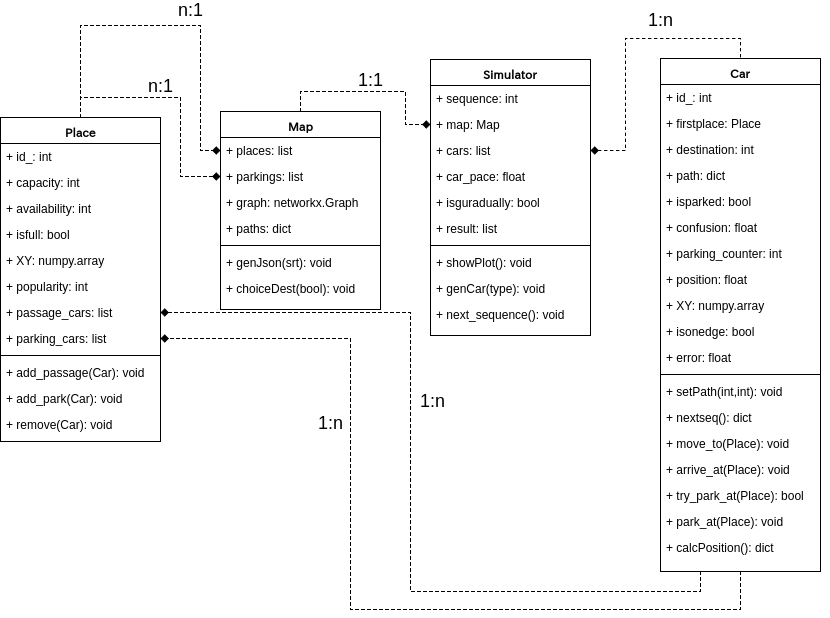
\includegraphics[width=14cm]{fig/class_figure.png}
	\caption{本シミュレータの各クラスの関係性}
	\label{class-implementation-figure}
\end{figure}

\section{ネットワークモデルの推定}
\label{infer-networkmodel}
本実装では第\ref{proposal}章で述べた提案手法を用いて,得られた位置情報のログデータを解析し,以下の3点についての自律的な推定を行う.
\subsection{駐車区画座標の推定手法}
\label{infer_parking_position}
本シミュレータ上の仮想車両が駐車をした際の座標群を,石岡らによる提案手法\cite{Ishioka}を一部改良した分類手法に基づいてクラスタリングする.各クラスタの重心となる点を駐車区画の中心地点の座標と推定する.
\subsubsection{用いる実装}
すべての位置情報ログデータから$Park$フラッグが付与されたログを抽出し,X-Means法\cite{Pelleg}を用いてクラスタリングする.
本実装では石岡らによる手法\cite{Ishioka}をPython\footnote{オブジェクト指向プログラミング言語とその実行環境.\url{https://www.python.org/}}環境に対応させたYuichi Goto(yasaichi)氏の実装\cite{Yasaichi}\cite{Yasaichi-git}を一部改良して用いる.
改良点は以下の2点である.これによりクラスタリング中の例外発生を防止することが出来る.
\begin{itemize}
	\item 共分散行列の利用 \\
	      Goto氏による実装\cite{Yasaichi-git}ではBIC(ベイズ情報量基準)を求める際の指標として,不偏共分散を利用している.
	      n組のデータ($x_1$,$y_1$),($x_2$,$y_2$) $\cdots$ ($x_n$,$y_n$)が存在するとき,不偏共分散$s_{xy}$は以下のように示すことが出来る.\\
	      \begin{align}
	      	s_{xy} = \frac{1}{n - 1} \displaystyle \sum_{i = 1}^n 
	      	{(x_i - \overline{x})(y_{i} - \overline{y})}          
	      \end{align}
	      不偏共分散は母集団全てを計算に用いることが出来ない場合に有効性を発揮する指数であるが\cite{Kyoubunsan-vs-huhenkyoubunsan},本手法ではそのクラスター全てのデータを算出に利用するため,必ずしも不偏共分散を利用する必要がない.
	      また,本環境では再帰的にクラスタリングを実行する際に,クラスタ内のデータの個数$n$が$1$になる場合がある.そのため,本実装では以下の式で表される共分散$s'_{xy}$を用いる.\\
	      \begin{align}
	      	s'_{xy} = \frac{1}{n} \displaystyle \sum_{i = 1}^n 
	      	{(x_i - \overline{x})(y_{i} - \overline{y})}       
	      \end{align}
	\item 尤度を求める際に特異共分散行列を許可する \\
	      前述の通り,本環境ではクラスタリングを実行する際にクラスタ内のデータの個数$n$が$1$になる場合がある.この時,共分散行列$s'_{xy}$は特異行列となる.本実装で用いた対数尤度関数\footnote{Python環境で動作する数値計算ライブラリSciPyのstats.multivariate\_normal関数\url{https://docsscipy.org/doc/scipy-0.14.0/reference/generated/scipy.stats.multivariate_normal.html}}はデフォルトで特異行列を許可しないためプログラムが異常終了する.
	      そのため,本実装では対数尤度関数に特異共分散行列を許可する引数を与える.
\end{itemize}

\subsection{駐車区画の有する駐車枠数の推定手法}
すべての位置情報ログデータから,$Park$フラッグと$Departure$フラッグが付与されたログを抽出し,各駐車区画の最大駐車台数を計数し,その区画の有する駐車枠数とする.サンプルとした時間$\max\{t\}$中にこの駐車区画が満車状態になる場合にのみ,正しい駐車枠数を推定することが出来る.
\subsubsection{用いる実装}
本実装では$Simulator$クラスのクラスメソッドに$infer\_parking\_slot$関数を用意した.以下に手順の概略を示す.

\begin{enumerate}
	\item 引数を与える.\\
	      すべての位置情報ログデータが挿入されている配列$all\_result$と,第\ref{infer_parking_position}項で求められた駐車区画の座標群$parking\_positions$を引数として与える.
	\item 推測された駐車区画群を示す配列$parkings$を作成する.\\
	      要素には駐車区画を表す辞書型のオブジェクトを挿入する.この辞書は仮識別子$id\_$,座標$position$,駐車枠数$capacity$,駐車している車両数$cars$のキーを有する.$capacity$,$cars$には初期値$0$を挿入する.
	\item 位置情報ログデータの走査 \\
	      すべての位置情報ログデータ$all\_result$を走査する.$Parking$フラッグを確認した際には該当する駐車区画の辞書の要素に対して$cars = cars + 1$を行い,$Departure$フラッグが確認された場合には$cars = cars - 1$を行う.
	\item $cars$要素の最大値を$capacity$に代入する.\\
	      前述の走査中に合わせて$cars$の最大値を記録する.すべての走査が終了した際に$cars$の最大値を$capacity$に代入する.
\end{enumerate}


\subsection{駐車区画$\cdot$交差点間を結ぶ道路の推定手法}
Edelkamp氏が提案したk-Means法をベースとした手法\cite{Edelkamp}を用いることを想定する.
全ての位置情報ログから駐車時以外のログを抜粋した位置情報群をX-Means法にてクラスタリングした際の各クラスターの中心点を結びフィッティングを行う.
各エッジの重みに関しては位置情報ログから車両の移動にかかるシーケンスを算出し,統計的危険値を取り除いた後の平均値とする.

なお,本論文ではBiagino氏らの評価実験\cite{Biagioni}によって有効性が示されているため,評価実験の対象から除外する.

\section{実装環境}
本説では本シミュレータの実行環境について記述する.

本シミュレータ及び推定システムはPython3\footnote{2018年1月現在,Python言語の現行仕様バージョンはPython3と呼ばれる.\url{https://www.python.org/}}とそのライブラリ群を用いて実装した.

図\ref{exec-enviroment}は第\label{evaluation}章で記述する評価実験を実行した環境を表している.
\begin{table}[htbp]
	\centering
	\begin{tabular}{llr}
		\hline
		\multicolumn{3}{c}{実行環境}                                                                               \\ \hline
		\multicolumn{2}{l}{ソフトウェア} & \multicolumn{1}{c}{バージョン}                                                 \\ \hline
		\multicolumn{2}{l}{Python} & 3.6.2(Anaconda3-5.0.0)                                                    \\
		  & NumPy \protect \footnotemark[5]                                                        & 1.13.1                                                                    \\
		  & NetworkX \protect \footnotemark[6]   & 1.11                                                                      \\
		  & GeoPy \protect \footnotemark[7]  & 1.11.0                                                                    \\
		  & SciPy \protect \footnotemark[8]                                                                                    & 8.99                                                                      \\
		  & matplotlib \protect \footnotemark[9]                                          & 2.0.2                                                                     \\
		  & setproctitle \protect \footnotemark[10]                            & 1.11.10                                                                   \\
		  & XMeans                                                                                                                                                        & \multicolumn{1}{l}{https://gist.github.com/yasaichi/254a060eff56a3b3b858} \\ \hline
		\multicolumn{2}{l}{ハードウェア} & \multicolumn{1}{c}{チップセット}                                                    \\ \hline
		  & HP ProLiant DL320e Gen8 v2                                                                                                                                    & \multicolumn{1}{l}{Intel(R) Xeon(R) CPU E3-1240 v3 @ 3.40GHz}             
	\end{tabular}
	\label{exec-enviroment}
	\caption{シミュレータの実行環境}
\end{table}
\footnotetext[7]{数学的な計算や行列式に用いるライブラリ.\url{http://www.numpy.org/}}
\footnotetext[8]{ネットワークグラフの構築や描写,最短経路の計算などに用いるライブラリ.\url{https://networkx.github.io/}}
\footnotetext[9]{地球上の座標を扱うためのライブラリ.本実装では座標間の距離計算に用いた.\url{https://github.com/geopy/geopy}}
\footnotetext[10]{数値計算用ライブラリ.\url{https://www.scipy.org/}}
\footnotetext[11]{ネットワークグラフや図表のプロットを行う.\url{https://matplotlib.org/}}
\footnotetext[12]{実行中のプロセス名を変更するライブラリ.\url{https://github.com/dvarrazzo/py-setproctitle}}